\documentclass[main.tex]{subfiles}

\begin{document}
\begin{titlepage}
\thispagestyle{empty}

% --- KHUNG VIỀN ---
\noindent
% --- KHUNG VIỀN ---
\noindent
\begin{tikzpicture}[remember picture, overlay]
    \node[inner sep=0pt] at (current page.center) {
        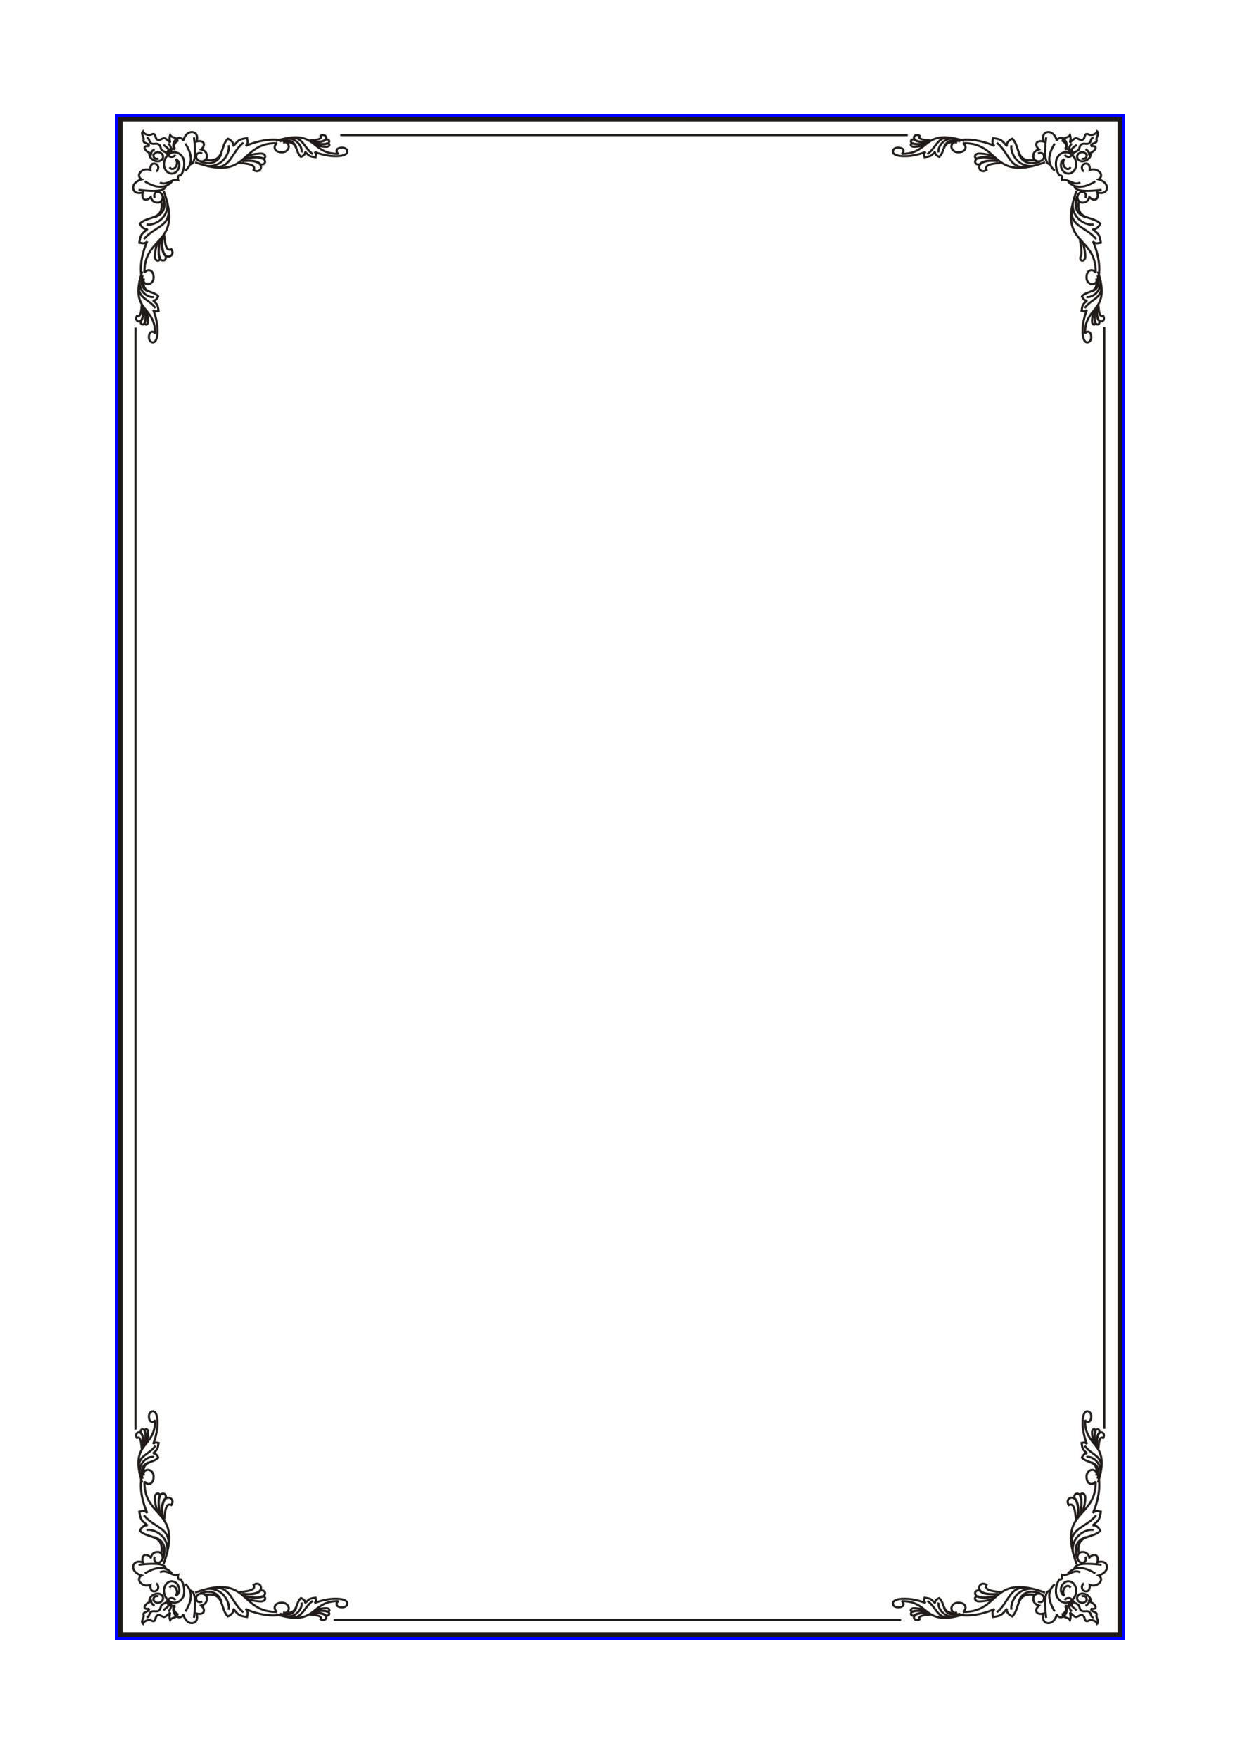
\includegraphics[]{img/frame.pdf} 
    };
\end{tikzpicture}%

\begin{spacing}{1}
\begin{center}
    % --- TIÊU ĐỀ ---
    \vspace*{1cm} % Khoảng cách từ viền trên xuống
    {\large \textbf{HỌC VIỆN CÔNG NGHỆ BƯU CHÍNH VIỄN THÔNG}} \\[0.1cm]
    {\large \textbf{KHOA CÔNG NGHỆ THÔNG TIN 1}} \\[0.1cm]
    {\large \textbf{\underline{\hspace{3cm}} o0o}} 
    \underline{\hspace{3cm}}\\
    
    \vfill
    
    % --- LOGO ---
    
\includegraphics[width=4.5cm]{img/ptit_logo.png} \\ 
    
    \vfill 
    
    % --- TÊN TIỂU LUẬN ---
    {\LARGE \textbf{TIỂU LUẬN VERSION 1}} \\
    {\LARGE \textbf{KIẾN TRÚC VÀ THIẾT KẾ PHẦN MỀM}} \\
    \vfill 
    
    % --- THÔNG TIN SINH VIÊN ---
    \begin{tabular}{ll}
        \textbf{Giảng viên hướng dẫn\hspace{0.5cm}} & \textbf{PGS.TS Trần Đình Quế} \\[0.3cm]
        \textbf{Họ và tên sinh viên} & \textbf{Trần Đức Trung} \\[0.3cm]
        \textbf{Mã sinh viên} & \textbf{B22DCCN875} \\[0.3cm]
        \textbf{Lớp} & \textbf{D22CNPM06} \\[0.3cm]
        \textbf{Nhóm} & \textbf{8}
    \end{tabular}

    \vfill
    \vfill % Tăng khoảng trống để đẩy phần dưới cùng xuống
    
    % --- ĐỊA ĐIỂM ---
    {\textit{\textbf{Hà Nội, 2026}}}
    \vspace*{1cm} % Khoảng cách từ chữ Hà Nội xuống viền dưới
\end{center}
\end{spacing}
\end{titlepage}
\end{document}